\chapter{Week9}
\section{Friday}\index{week8_Thursday_lecture}
We are now in the multi-variate differentiation part. 
\paragraph{Comments on question in last lecture}
The question left in the last lecture is that
\begin{quotation}
In dimension $\mathbb{R}^k$ with $k$ to be determined, is it possible to find the smallest $k$ such that a sphere $S^2$ and a circle $S^1$ have a way of putting to make each point from $S^2$ to $S^1$ have the same distance?
\end{quotation}
The answer is $k=5$, Let's give an example. We define the sphere and the circle to be 
\[
\begin{aligned}
S^2&=\{(x,y,z,0,0)\mid x^2+y^2+z^2=1\},\\
S^1&=\{(0,0,0,u,v)\mid u^2+v^2=1\}
\end{aligned}
\]
Therefore, the distance between any two points on the sphere and the circile, respectively, is
\[
d=\sqrt{x^2+y^2+z^2+u^+v^2}\equiv\sqrt{2}
\]
Why $k\le 4$ is not ok? Now we give a instructive proof:
\begin{proof}
For the case $k\le4$, let $\bm c_2$ denote the center of sphere $S^2$ with radius $r_2$; $\bm c_3$ deote the center of circle $S^1$ with radius $r_1$. Any point on $S^2$ can be written as $\bm c_2+\bm x$ with $\bm x\in M:=\{\bm x\in\mathbb{R}^3:\|\bm x\|=r_2\}$; and any point on $S^1$ can be written as $\bm c_1+\bm y$ with $\bm x\in N:=\{\bm y\in\mathbb{R}^2:\|\bm y\|=r_1\}$. It follows that the distance between any two points can be expressed as:
\[
d(\bm c_2+\bm x,\bm c_1+\bm y)=
\|(\bm c_2+\bm x) - (\bm c_1+\bm y)\|
=
\|\bm x\|^2+\|\bm c_2-\bm y-\bm c_1\|^2+2\inp{\bm x}{\bm c_2-\bm y-\bm c_1}
\]
Note that the distance between any point in $S^2$ and any point in $S^1$ is the same. In particular, $d(\bm c_2+\bm x,\bm c_1+\bm y)=d(\bm c_2-\bm x,\bm c_1+\bm y)$, which implies $\inp{\bm x}{\bm c_2-\bm y-\bm c_1}=0,\forall\bm x\in M,\bm y\in N$, i.e., 
\[
\bm c_2-\bm c_1+N\subseteq M^\perp,
\]
and therefore
\begin{align*}
\dim(\bm c_2-\bm c_1+N)&=\dim(N)=2\\
&\le\dim(M^\perp)=k-3,
\end{align*}
i.e., $k\le 5$ is the sufficient condition of the problem.

\end{proof}


\subsection{Preliminaries}
\paragraph{Notations}Here we use lower-case and bolded alphabet to denote a vector, e.g., $\bm x$; upper-case and bolded alphabet to denote a matrix, e.g., $\bm A$; unbolded alphabet to denote a scalar, e.g., $x_1$ or $A_1$

Define $\bm x:=(x_1,\dots,x_m)$ and $\bm y:=(y_1,\dots,y_m)$, we define the $L_2$ norm
\begin{align*}
d(\bm x,\bm y):&=\|\bm x-\bm y\|\\
&=\left[(x_1-y_1)^2+\cdots+(x_m-y_m)^2\right]^{1/2}
\end{align*}
and the $L_1$, $L_{S}$ (sup) norm:
\begin{align*}
d_1(\bm x,\bm y):&=\|\bm x-\bm y\|:=|x_1-y_1|+\cdots+|x_m-y_m|\\
d_S(\bm x,\bm y):&=\|\bm x-\bm y\|_S:=\max_{1\le i\le m}(x_i-y_i)
\end{align*}
\begin{definition}[Vector Norm]
A norm $\|\cdot\|$ is a function from a vector space $X$ to $\mathbb{R}$ such that
\begin{enumerate}
\item
$\|\bm x\|\ge0$, $\forall x\in X$; and $\|\bm x\|=0$ iff $\bm x=\bm0$;
\item
$\|\lambda\bm x\| = |\lambda|\|\bm x\|$, for $\forall x\in X,\lambda\in\mathbb{R}$;
\item
$\|\bm x_1+\bm x_2\|\le \|\bm x_1\| + \|\bm x_2\|$
\end{enumerate}
\end{definition}
\begin{remark}
Any norm defines a metric: $d(\bm x,\bm y)=\|\bm x-\bm y\|$. From now on, we pre-assume the norm to be $L_2$ norm and the metric to be $L_2$ metric, unless specified.
\end{remark}

The norm are used to masure the length of a vector, or the distance of two vectors. Correspondingly, the inner product can be used to measure the angle between two angles:
\begin{definition}[Inner Product]
An \emph{inner product} is a binary operation function $\inp{\cdot}{\cdot}: X\times X\mapsto\mathbb{R}$ such that
\begin{enumerate}
\item
$\inp{x}{x}\ge0$ for $\forall x\in X$ and $\inp{x}{x}=0$ iff $\bm x=0$
\item
$\inp{\bm x}{\bm y}=\inp{\bm y}{\bm x}$, for $\forall \bm x,\bm y\in X$
\item
$\inp{\lambda\bm x}{\bm y}=\lambda\inp{\bm x}{\bm y}$ for $\forall x,y\in X$ and $\forall \lambda\in\mathbb{R}$
\item
$\inp{x+y}{z}=\inp{x}{z}+\inp{y}{z}$
\end{enumerate}
\end{definition}
 \begin{remark}
 \begin{enumerate}
\item
 Any inner product always defines a norm, i.e., $\|\bm x\|=\sqrt{\inp{\bm x}{\bm x}}$.
 \item
The angle $\theta$ between vector $\bm x,\bm y$ is defined as:
\[
\theta = \cos^{-1}\left(\frac{\inp{\bm x}{\bm y}}{\|\bm x\|\|\bm y\|}\right)
\]
In particular, $\bm x$ and $\bm y$ are orthogonal, i.e., $\inp{\bm x}{\bm y}=0$ if $\theta=\pm\frac{\pi}{2}$; $\bm x,\bm y$ are parallel if $\theta=0,$ or $\theta=\pm\pi$.
\end{enumerate}
 \end{remark}
\subsection{Differentiation}
\paragraph{Review for One-dimension}
Given a function $f:\mathbb{R}\mapsto\mathbb{R}$, the derivative is defined as
\[
f'(x_0)=\lim_{x\to x_0}\frac{f(x) - f(x_0)}{x-x_0}
\]
or equivalently, the value $f'(x_0)$ is said to be the derivative of $f$ if it satisfies the equality:
\begin{align*}
0&=
\lim_{x\to x_0}\left[\frac{f(x) - f(x_0)}{x-x_0} - f'(x_0)\right]\\
&=
\lim_{x\to x_0}\frac{f(x) - f(x_0) - f'(x_0)(x-x_0)}{x-x_0}\\
&=
\lim_{x\to x_0}
\left|
\frac{
f(x) - [f(x_0) + f'(x_0)(x-x_0)]
}{x-x_0}
\right|
\end{align*}
The interpretation is that the affine (linear function) $f(x_0)+f'(x_0)(x-x_0)$ approximates $f$ near $x_0$ in at least first order. We can use the similar way to define the high-dimension derivative.
\paragraph{High-Dimension Derivative}
\begin{definition}[Differentiable]
A map $f:U\mapsto\mathbb{R}^n$, where $U$ is open in $\mathbb{R}^m$, is \emph{differentiable} at $\bm x_0\in U$ if
\begin{equation}
\lim_{\bm x\to\bm x_0}
\frac{
\left\|
f(\bm x) - f(\bm x_0) - \bm L(\bm x_0)(\bm x-\bm x_0)
\right\|
}{
\left\|
\bm x-\bm x_0
\right\|
}=0,
\end{equation}
where $\bm L(\bm x_0)$ is said to be the derivative of $f(\bm x)$ at $\bm x=\bm x_0$, which is often denoted as $Df(\bm x_0)$, or $f'(\bm x_0)$.
\end{definition}
\begin{remark}
Note that $f(\bm x),f(\bm x_0)\in\mathbb{R}^n$, but $(\bm x-\bm x_0)\in\mathbb{R}^m$, thus $L(\bm x_0)$ is a \emph{linear transformation} from $\mathbb{R}^m$ to $\mathbb{R}^n$, i.e., a $n\times m$ matrix. 
\end{remark}
\paragraph{Interpretation}
We re-write $f(\bm x): \mathbb{R}^m\mapsto\mathbb{R}^n$ (a $n$-vector valued function of a $m$-vector argument) as:
\[
\begin{array}{l}
f(\bm x)=\begin{pmatrix}
f_1(\bm x)&\cdots&f_n(\bm x)
\end{pmatrix},
\end{array}
\]
with each $f_i:\mathbb{R}^m\mapsto\mathbb{R}$ being a scalar-valued function of a $m$-vector argument. Let's study only one component with $2$-argument function first, i.e., $n=1,m=2$. 
\begin{figure}[H]
\centering
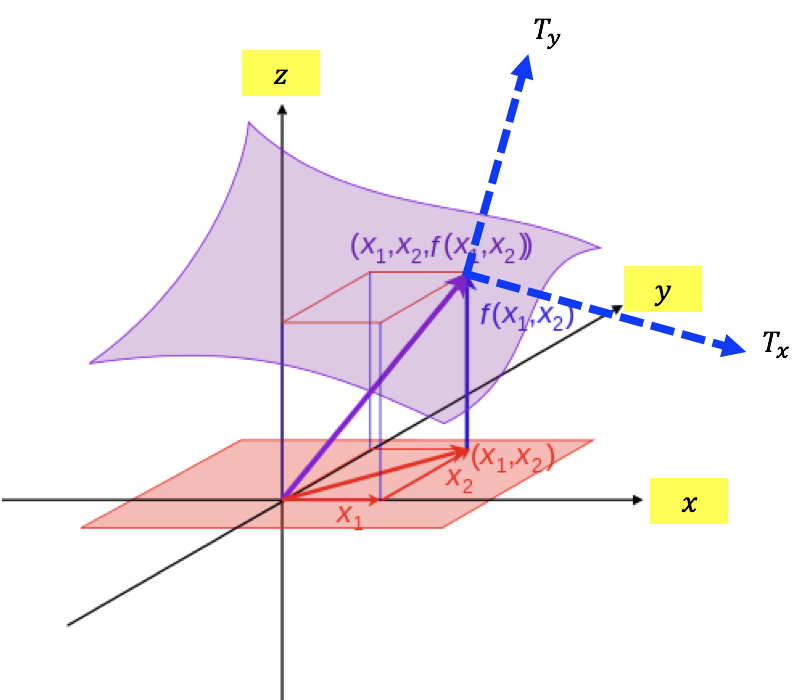
\includegraphics[width=10cm]{week9/f_9_1}
\caption{Diagram for partial derivatives}
\end{figure}
Given a surface $S:z=f(x_1,x_2)$, we study a point on the surface $S$, say $M_0(x_1,x_2,f(x_1,x_2))$. If the surface $S$ intersects the plane $y=x_2$  with the point $M_0$, then the \emph{partial derivative} $\frac{\partial f}{\partial{x_1}}(x_1,x_2)$ denotes the slope of the tangent line at $M_0$; the tangent line $T_{x_1}$ can be denoted as a vector $T_{x_1}:=(1,0,\frac{\partial f}{\partial{x_1}}(x_1,x_2))$. 

Similarly, if the surface $S$ intersects the plane $x=x_1$  with the point $M_0$, then $\frac{\partial f}{\partial{x_2}}(x_1,x_2)$ denotes the slope of the tangent line at $M_0$; the tangent line $T_{x_2}$ can be denoted as a vector $T_{x_2}:=(0,1,\frac{\partial f}{\partial{x_2}}(x_1,x_2))$. 

Furthermore, the plane $\Span\{T_{x_1},T_{x_2}\}$ denotes the tangent plane at point $M_0$.
\begin{corollary}\label{Cor:9:1}
$f$ is differentiable at $\bm x_0$ implies all partial derivatives of $f$ at $\bm x_0$ exist.
\end{corollary}
The converse is not true. Let's raise a counter-example to explain that.
\begin{example}
\[
f(x_1,x_2)=\left\{
\begin{aligned}
\frac{x_1x_2}{x_1^2+x_2^2},&\quad (x_1,x_2)\ne(0,0)\\
0,&\quad (x_1,x_2)=(0,0)
\end{aligned}
\right.
\]
When $x_2=mx_1$, we have
\[
f(x_1,mx_1) = \frac{mx_1^2}{x_1^2+mx_1^2}=\frac{m}{1+m^2},
\]
i.e., $f$ is not differentiable at the origin as it is not continuos at the origin.

However, we can verify that $\frac{\partial f}{\partial x_1}(0,0)=0=\frac{\partial f}{\partial x_2}(0,0)$.

\end{example}
What guarntees $f$ to be differntiable if all partial derivatives exist?
\[
\frac{\|f(\bm x) - f(\bm x_0) - Df(\bm x_0)(\bm x-\bm x_0)\|}{\|\bm x-\bm x_0\|}\to0,
\]
where $f:\mathbb{R}^m\mapsto\mathbb{R}^n$ and $Df(\bm x_0)$ be a $n\times m$ matrix. We re-write the formula for the derivative of $f$ at $\bm x=\bm x_0$ first. Here we write $f(\bm x_0)$ in column vector form:
\begin{equation}\label{Eq:9:2}
\begin{pmatrix}
f_1(\bm x)\\
f_2(\bm x)\\
\vdots\\
f_n(\bm x)
\end{pmatrix}=
\begin{pmatrix}
f_1(\bm x_0)\\
f_2(\bm x_0)\\
\vdots\\
f_n(\bm x_0)
\end{pmatrix}
+
\begin{pmatrix}
\frac{\partial f_1}{\partial x_1}(x_0)&\frac{\partial f_1}{\partial x_2}(x_0)&\cdots&\frac{\partial f_1}{\partial x_m}(x_0)\\
\frac{\partial f_2}{\partial x_1}(x_0)&\frac{\partial f_2}{\partial x_2}(x_0)&\cdots&\frac{\partial f_2}{\partial x_m}(x_0)\\
\vdots&\vdots&\ddots&\vdots\\
\frac{\partial f_n}{\partial x_1}(x_0)&\frac{\partial f_n}{\partial x_2}(x_0)&\cdots&\frac{\partial f_n}{\partial x_m}(x_0)\\
\end{pmatrix}
\begin{pmatrix}
x_1- x_{0,1}\\
x_2- x_0\\
\vdots\\
x_m- x_0\\
\end{pmatrix}
+o(\|\bm x-\bm x_0\|),
\end{equation}
where $o(\|\bm x-\bm x_0\|)$ is a $m\times 1$ vector that has order less than $\|\bm x-\bm x_0\|$.

Each entry in LHS of (\ref{Eq:9:2}) can be expressed as:
\[
f_i(\bm x)=f_i(\bm x_0)+\nabla\trans f_i(\bm x_0)\cdot (\bm x-\bm x_0)+o(\|\bm x-\bm x_0\|),
\]
with $\nabla\trans f_1(\bm x_0) = \begin{pmatrix}
\frac{\partial f_1}{\partial x_1}(\bm x_0)
&
\cdots
&
\frac{\partial f_1}{\partial x_m}(\bm x_0)
\end{pmatrix}$ to be a row vector, and $(\bm x-\bm x_0)$ to be a column vector.

\paragraph{Sufficient Condition for differentiability}
Recall that we have faced a function that is everywhere differentiable but nowhere monotone, which is very counter-inuitive. If adding the condition that such function is continuously differentiable, then such function is monotone. Similarly, the gap for corollary(\ref{Cor:9:1}) is continuous differentiability.
\begin{theorem}
Let $f:U\mapsto\mathbb{R}^n$, where $U\subseteq\mathbb{R}^m$ is open. If all partial derivatives of $f$ are \emph{continuous} in $U$, then $f$ is differentiable in $U$.
\end{theorem}
\begin{proof}[Proof for $n=2,m=1$ case]
Consider $f:\mathbb{R}^2\mapsto\mathbb{R}$, for $x_0\in U$ with small $h,k$, we have:
\begin{subequations}
\begin{align}
f(x_0+h,y_0+k) - f(x_0,y_0)&=[f(x_0+h,y_0+k) - f(x_0+h,y_0)] + [f(x_0+h,y_0) - f(x_0,y_0)]\\
&\mbox{(by Mean Value Theorem, $\exists (c,d)\in[0,h]\times[0,k]$ such that)}\\
&=k\frac{\partial f}{\partial y}(x_0+h,y_0+c) + h\frac{\partial f}{\partial x}(x_0+d,y_0)\\
&=k\frac{\partial f}{\partial y}(x_0,y_0+c)+o(h)+h\frac{\partial f}{\partial x}(x_0,y_0)+o(h)\\
&=k\frac{\partial f}{\partial y}(x_0,y_0)+h\frac{\partial f}{\partial x}(x_0,y_0)+o(h)+o(k)
\end{align}
\end{subequations}
Or we write it in compact matrix form:
\[
f(x_0+h,y_0+k)=f(x_0,y_0)+\begin{pmatrix}
\frac{\partial f}{\partial x}(x_0,y_0)&
\frac{\partial f}{\partial y}(x_0,y_0)
\end{pmatrix}\begin{pmatrix}
h\\k
\end{pmatrix}+o(\|(h,k)\|),
\]
i.e., the derivative of $f$ at $x=x_0$ exists, say $(\frac{\partial f}{\partial x},\frac{\partial f}{\partial y})$. Thus $f$ is differentiable.
\end{proof}
The same proof can easily extend to $f:\mathbb{R}^n\mapsto\mathbb{R}$ by adding and subtracting $n-1$ terms and then apply mean value theorem for $n$ times; the extension to $f:\mathbb{R}^n\mapsto\mathbb{R}^m$ is clear by the same proof for each component.






\begin{proof}
Consider in general $f:\mathbb{R}^n\mapsto\mathbb{R}^m$, and it suffices to show (\ref{Eq:9:2}), and moreover, it suffices to show each entry $f_i(\bm x)$ in (\ref{Eq:9:2}) can be expressed as
\[
f_i(\bm x)=f_i(\bm x_0)+\nabla\trans f_i(\bm x_0)\cdot (\bm x-\bm x_0)+o(\|\bm x-\bm x_0\|).
\]
Let's abuse notation to refer $g$ as the $i$-th entry of $f_i$, i.e., $g:\mathbb{R}^n\mapsto\mathbb{R}$.

Let $\varepsilon>0$, by continuity of partial derivatives, we can pick $\delta>0$ such that for any $\|\bm h\|<\delta$, we have
\begin{equation}
\left\|\frac{\partial g}{\partial x_k}(\bm x+h) - \frac{\partial g}{\partial x_k}(\bm x) \right\|<\varepsilon,\qquad k=1,2,\dots,n
\end{equation}
Let $\bm L=(\frac{\partial g}{\partial x_1}(\bm x),\dots,\frac{\partial g}{\partial x_n}(\bm x))$; $\phi_k(\bm h)=(h_1,h_2,\dots,h_k,0,\dots,0)$, $\phi_0(\bm h)=\bm0$, and suppose $\|\bm h\|<\delta$,
, then we have:
\begin{align}
|g(\bm x+\bm h) - g(\bm x) - \bm L\bm h| &=\left|\sum_{k=1}^n[g(\bm x+\phi_k(\bm h)) - g(\bm x+\phi_{k-1}(\bm h)) - \frac{\partial g}{\partial x_k}(\bm x)h_k]\right|\\
&\le\sum_{k=1}^n\left|g(\bm x+\phi_k(\bm h)) - g(\bm x+\phi_{k-1}(\bm h)) - \frac{\partial g}{\partial x_k}(\bm x)h_k\right|
\end{align}
By the Mean Value Theorem, there exists $\bm c_k\in[\bm x+\phi_{k-1}(\bm h),\bm x+\phi_k(\bm h)]$ such that $g(\bm x+\phi_k(\bm h)) - g(\bm x+\phi_{k-1}(\bm h))=\frac{\partial g}{\partial x_k}(\bm c_k)h_k$, and therefore
\begin{align}
|g(\bm x+\bm h) - g(\bm x) - \bm L\bm h|&\le
\sum_{k=1}^n\left|\frac{\partial g}{\partial x_k}(\bm c_k)h_k - \frac{\partial g}{\partial x_k}(\bm x)h_k\right|\\
&=\sum_{k=1}^n\left|\frac{\partial g}{\partial x_k}(\bm c_k) - \frac{\partial g}{\partial x_k}(\bm x)\right||h_k|\\
&<\varepsilon\sum_{k=1}^n|h_k|\label{Eq:9:9}
\end{align}
where (\ref{Eq:9:9}) is due to the continuty of partial derivatives. To make life easier, we specify the norm to be $L_1$ norm, which follows that
\[
|g(\bm x+\bm h) - g(\bm x) - \bm L\bm h|\le\varepsilon\|\bm h\|_1,
\]
which implies $g$ is differentiable at $\bm x$. In paricular, if every component $f_i$ is differentiable, then $f$ is differentiable.

\end{proof}

\paragraph{Planning for following weeks}

The next lecture will talk about the chain rule, the inverse, the derivative of inverse, the directional derivative, the gradient. Next Friday will talk about Inverse function theorem and Implicit function theorem, which may last for two weeks.